\documentclass[conference]{IEEEtran}
\IEEEoverridecommandlockouts
% The preceding line is only needed to identify funding in the first footnote. If that is unneeded, please comment it out.
\usepackage{cite}
\usepackage{amsmath,amssymb,amsfonts}
\usepackage{algorithmic}
\usepackage{graphicx}
\usepackage{textcomp}
\usepackage{tabu}
\usepackage{multirow}
\usepackage{graphicx}
\usepackage{subfigure}
\usepackage{xcolor}
\usepackage[colorlinks,linkcolor=blue]{hyperref}
\usepackage{enumitem}
\newlist{subquestion}{enumerate}{1}
\setlist[subquestion,1]{label=(\alph*)}
\usepackage{listings}
\usepackage{pythonhighlight}
\usepackage{fancyhdr}
\usepackage{threeparttable}
% (1) choose a font that is available as T1
% for example:
\usepackage{lmodern}
\usepackage[T1]{fontenc}
% (3) load symbol definitions
\usepackage{textcomp}
\usepackage{booktabs}


\pagestyle{fancy}
\cfoot{\thepage}


% flowchart
\usepackage{tikz,mathpazo}
\usetikzlibrary{shapes.geometric, arrows}
\usepackage{flowchart}

\def\BibTeX{{\rm B\kern-.05em{\sc i\kern-.025em b}\kern-.08em
    T\kern-.1667em\lower.7ex\hbox{E}\kern-.125emX}}

\setcounter{page}{1}
\begin{document}

\title{The Voice of Customers  \\
\begin{large} 
  CFPB data analysis from 2005 by now
\end{large} 
}

\author{\IEEEauthorblockN{Danfeng Wang}
\IEEEauthorblockA{\textit{Big Data Analytics} \\
\textit{Letterkeney Institute of Technology }\\
Donegal, Ireland \\
L00162010@student.lyit.ie }

}

\maketitle

\begin{abstract}
   This is a customer complaint dataset about the financial product consumption in the USA. We would like to hear the voice from these customers by analysing it. How many valid complaint data in this dataset? What is the most concerned problem? What is the strongest voice of these complaints? Have those financial companies improved their service from this? Can we predict the trends of the complaints?
   With these questions, we are going to have a exploration to this dataset. Please take a deep breath, hear the voices from the customers. Let the millions of complaints records tell us the truth, charts never lie.
\end{abstract}


\section{Introduction}
In this project, we are going to analysis the consumers complaints about financial products in the USA. The dataset of this project obtained from the data.gov website which is collected by the Consumer Financial Protection Bureau, an agency of the United States government responsible for consumer protection in the financial sector \cite{datasource}. It includes complaints dating from 2015 by now. 

The volume of this dataset is roughly 2 million items. We apply big data analytic related techniques, such as machine learning, natural language process (NLP) and so force, to achieve the goal of the project:

\begin{enumerate}[label=(\roman*)]
\item providing descriptive analysis combined with visualization, such as bar charts and word cloud charts, to give an insight and summarization of these data.
\item providing prediction model by machine learning approaches.
\end{enumerate}


%The analysis of this dataset can be used for  finding common problems of products in financial sector and making precautions. By using data visualization and machine learning approach, this report gives insights and understanding into consumers perspective so that to provide ideas of how to improve control measures in financial products or give better regulations and decisions in the management of the financial market. %
\begin{itemize}
\item What's the most complained from different dimensions, such as complained channels,companies, products. Have they changed over time?

\item Pictures speak louder than text, what can we get from the narrative of those complaints.

\item Can we predict the issue type? Can we predict the process result to guide the urgency of these complaints, so that the companies can give a  higher priority when dealing with the urgent complaints.
\item The quality of service - responding time, where, what and which providers got the most complaints. Any improvement later? 

\end{itemize}

\section{Code list}

\section{System preparation}\label{AA}
We apply big data and machine learning related techniques to implement this project. 

In the process of achieving the above goal, we have three aspects to consider:

\textbf{Data engineering
}\begin{itemize}
\item  - data ingestion
\item - data preparation 
\item - visualization
\end{itemize}


\textbf{Machine learning
}\begin{itemize}
\item  - data loading
\item - feature engineering
\item - training and prediction
\item - model tuning 
\end{itemize}







Databrick is a cloud platform for big data analysis. In this project, we use Databrick as the data storage, analysis and modelling platform.
Follow the next steps for system preparation.
\begin{itemize}

\item Sign up for a free Databrick trial.
\item Create a cluster 6.4 (includes Apache Spark 2.4.5, Scala 2.11) 
\item Create notebook.
\item Start cluster.
The cluster will be terminated automatically after 60 minutes of inactivity.
\end{itemize}

At the data modelling stage, we use MLFlow on Databrick to implement the machine learning pipeline. MLFlow is an platform for managing the machine learning lifecycle.  


\section{Dataset acquisition}



\begin{itemize}
\item Download dataset file from the web site.
\item Upload the file into DBFS. 
\item Unzip and load the data into table.
\item Check the integrity.
\end{itemize}
During this process, we found the csv format cannot be correctly loaded by spark SQLContext, . By reading few line from the file, we found the fields are seperated by comma, one of the descriptive field \emph{Consumer complaint narrative} is enclosed by double quotes. By applying loading parameters such as \emph{escape} and \emph{quotion}, the problem remained.
In order to avoid this problem, we tried loading json file.

\subsection{Fields description}\label{AA}
see Table1.
\begin{itemize}
\item \textit{Company public response} - standard items. This is how the company attributed the complaint. Some are believed the company should not be responsible for the issue, it should be a third party, policy, consumer, misunderstanding and so forth. Some are resolved privately which we can not distinguish the attribute, and some are believed invalid complaints.
\item \textit{Company response to consumer} - The process status is close, in progress or untimely response in which the close status has several different way including close with explanation, monetary relief, non-monetary relief, relief or without relief. We can see percentage of issue resolved and in which way the issues have been resolved.  
%\item \textit{Product} - Does the products complained distributed evenly? Which products are the most complained? Are the products complained by consumers changed within these years, and whether the changes are influenced by the complaints data..

\end{itemize}
\begin{table}[h]
\caption{Dataset}
\begin{threeparttable}
\begin{tabular}{p{1.2cm}|p{4cm}|p{2.3cm}}
\hline
\hline
Category\tnote{1} & Column name & Description\tnote{2} \\ \hline
identity & complaint\_id & numeric string  \\ \hline

\multirow{4}{*}{company} & company & string \\ \cline{2-3} 
						 & date\_sent\_to\_company & yyyy\-mm\-dd \\ \cline{2-3}
                         & company\_public\_response &  \\ \cline{2-3} 
                         & company\_response & category \\ \cline{2-3} 
                         & consumer\_consent\_provided & category  \\ \cline{2-3} 
                         & timely   & yes/no \\ \hline
\multirow{2}{*}{product} & product & string \\ \cline{2-3}
 						 & sub\_product  & string \\ \hline
\multirow{6}{*}{consumer} 
                       & submitted\_via   & channel/category \\ \cline{2-3}
					   & issue  & category \\ \cline{2-3}
					   & sub\_issue  & \\ \cline{2-3}
					   & complaint\_what\_happened	  & long text \\ \cline{2-3}
					   & tags	  & string \\ \cline{2-3}
                       & consumer\_disputed  & yes/no \\ \cline{2-3}
                       & state   & category / geo  \\ \cline{2-3}
                       & zip\_code & category / geo  \\ \hline                         
\bottomrule
\end{tabular}
\begin{tablenotes}
\footnotesize
\item[1] The business purpose of the column.
\item[2] The column type and other description.

\end{tablenotes}
\end{threeparttable}
\end{table}

	\begin{figure}[h]
		\centering
		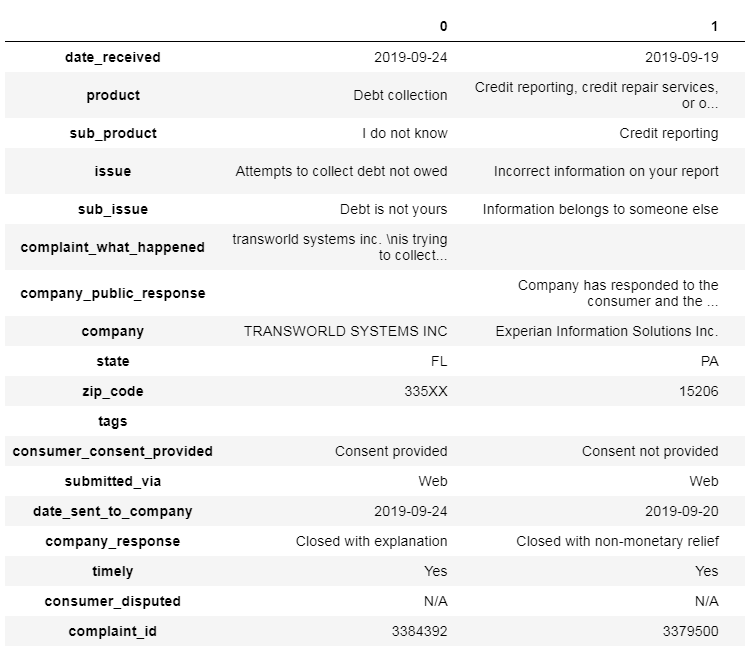
\includegraphics[width=1\linewidth]{img/data2rows.png}
\caption{sample data} \label{fig:sample data}
	\end{figure} 

\subsection{Business process}\label{AA}
The complaint data will go through the following steps when it is submitted to the CFPB, see Figure 1.

 % basic shape of the flowchart
\usetikzlibrary{shapes.geometric,arrows}

\tikzstyle{decision} = [ diamond, draw, fill=blue!20, text width=4.5em, text badly centered, node distance=3cm, inner sep-0pt]  
\tikzstyle{block} = [ rectangle, draw, fill=blue!20, text badly centered, rounded corners, minimum height=3em]  
\tikzstyle{line} = [ draw, -latex']  
\tikzstyle{terminator} = [ ellipse, draw,fill=red!20, node distance=3cm, minimum height=3em]  

\begin{figure}
\centering
\begin{tikzpicture}[node distance=2cm, auto]  
  \node [terminator]           (a)  {complaint submitted};  
  \node [block, below of=a]  (b)  {review and route};  
  \node [block, below of=b]  (c) {company response};  
  \node [block, below of=c] (d) {complaint published};  
  \node [block, below of=d] (e) {consumer review};  
  
  \path [line] (a)  -- (b);  
  \path [line] (b)  -- (c);  
  \path [line] (c) -- (d);  
  \path [line] (d) -- (e); 
  \path [line] (e) edge[loop right] (); 
\end{tikzpicture}
\caption{data flow} \label{fig:data flow}
\end{figure}


\subsection{More about the data}\label{AA}
The complaint facts will not be verified by CFPB, but it gives the companies opportunity to confirm the consumer has commercial relationship with them. 



\section{Data preparation}\label{AA}
In order to make it easier to manipulate in the next stages, the dataset will be prepared as follows:

\subsection{Data integration}\label{AA}
The purpose of this stage is to make sure the dataset is analysable.

By looking at the data, 
\begin{itemize}
\item check null value to target fields.
\item validate the date fields.
\item Check the value of state fields.Standardizing?
\\item type conversion.
\\item eliminating meaningless words such as stop words, symbols, and convert the text into lower case.
\end{itemize}



\subsection{Data transformation}\label{AA}
\begin{itemize}

\item date: generate corresponding fields such as year, month, week and so forth.
\item location: generate geographical columns, such as longitude, latitude and so forth.
\item standardized text: convert text to code. Split the text into words, extract nouns.
\end{itemize}


\section{Descriptive analysis }

In this process, we visualized the data from different dimensions to see how many complaints happened, as well as the trend over time.

For example, the figure below shows the top 6 complained products by year. During the first 4 years, most complaints mainly focus on the mortgage (green bar), and the amount of complaints declined gradually after 2013 and remains static from 2018. While in 2017, the \textit{credit reporting} product (yellow bar) became the most-complained-about financial product, and it has been growing rapidly since then. 


\begin{figure}[h]
\centering
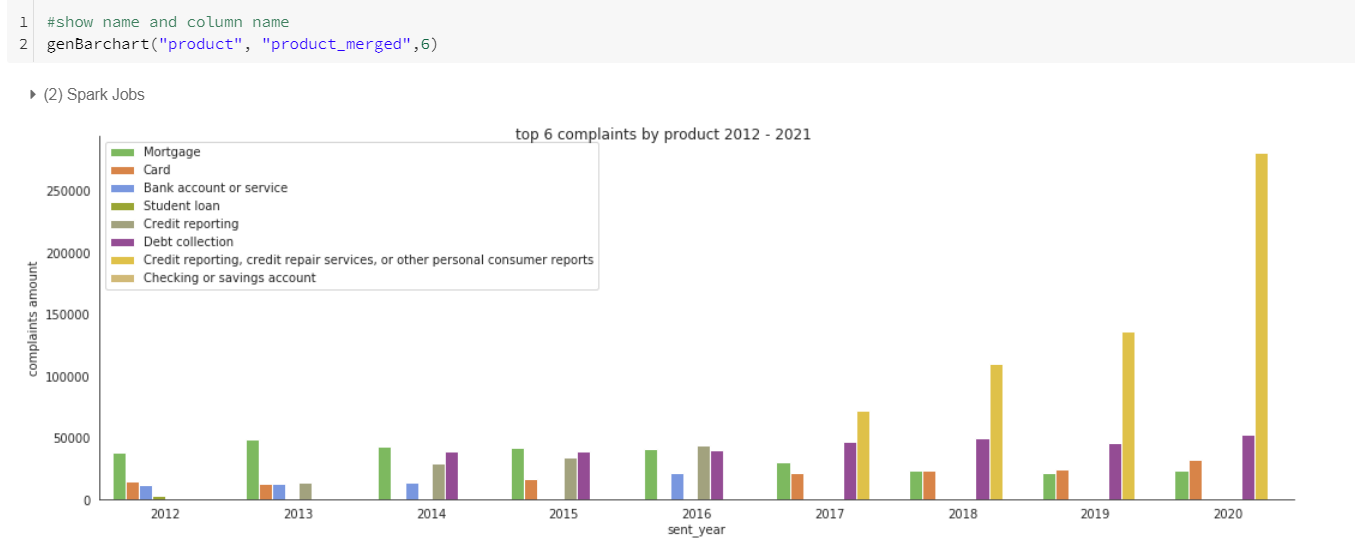
\includegraphics[width=1\linewidth]{img/byproduct.png}
\caption{top 6 complained product by year} \label{fig:xxxxx}
\end{figure} 


In this way, the complaints change over years can be shown by other dimensions, such as issue type, channel, companies, and so on and so forth. So functions have be defined here for further use.

\begin{figure}[h]
\centering
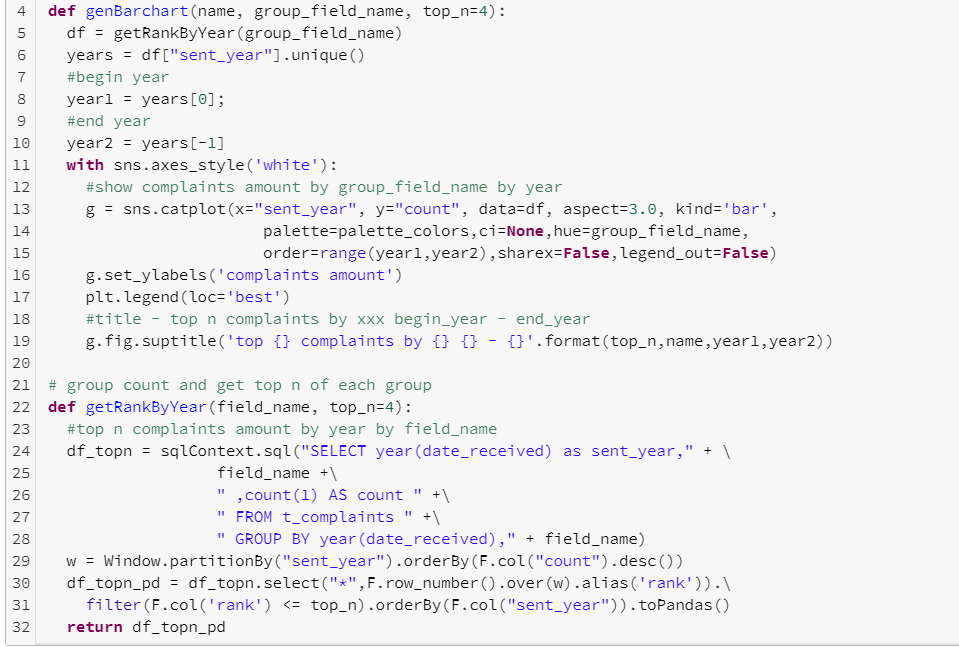
\includegraphics[width=1\linewidth]{img/chartfunction.png}
\caption{chart function} \label{fig:chartfunction}
\end{figure} 

\section{NLP}\label{AA}
As we listed in the \textit{table1}, the  \textit{complaint\_what\_happened} column is the consumer's narrative of the complaint. We apply NLP analysis to dig into this column for a deep insight.

The pipeline of dealing with NLP usually consists of several steps:

\begin{enumerate}
\item normalization - convert the text content into lower case and remove the non words such as punctuation and other non alphanumeric characters.
The private information of this column has been replaced by x with the corresponding length. In order to remove them, they were added into the stop words array.
\item tokenization - split the sentences into words by space.
\item stop words - remove meaningless words.
\item tagging - only keep specific word types, such as noun, adjective.
\item stemming - reducing the words to it's word stem so that the similar words lie under a same stem.
\end{enumerate}

A pipeline is created for achieving the above steps.

\begin{figure}[h]
\centering
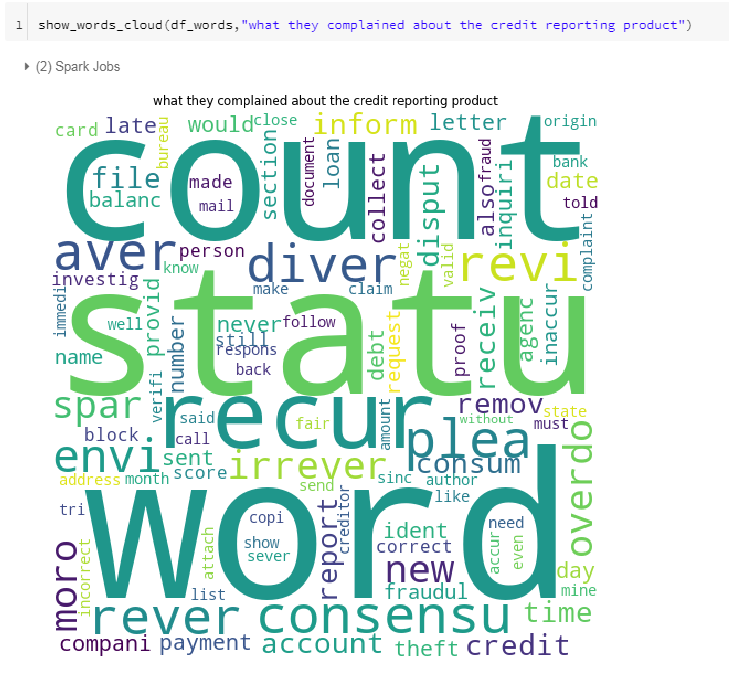
\includegraphics[width=0.9\linewidth]{img/word_cloud_reporting.png}
\caption{the voice of credit reporting product} \label{fig:wordcloudreporting}
\end{figure} 


\section{Predictive analysis }
When exploring this dataset, we found the part of within company response column, there are several ways for the company to deal with the issues. Some of the response involved with money or other non-monetary relief. It would be a valuable reference for the companies complained by the customers if we are able to predict the settlement whether involves with any forms of relief or not? 

In order to build predictive model to try to implement this task, we will follow the steps as below:
 
\textbf{Data preparation} - after the descriptive analysis stage, the dataset has been prepared and saved into database, we can use pyspark.sql api to retrieve data conveniently. For the narrative column, the sentences of that column has been processed by a nlp pipeline. 
 
\textbf{Feature engineering} - From the dataset introduction section, we have known that most of the features are nominal categorical data, such as issue, sub-issue, product, company response, and so force. We will convert these columns into numeric by applying one hot encoding and  create dummy variables of each categorical. By transforming these different values to columns, we can avoid the model regarding these numeric values as number instead of a specific category, because the number itself is meaningless\cite{feature_engineering}.


\textbf{Cross-validation} - we prepare the dataset by using 5-folder cross-validation. This is a popular method which tends to provide less biased model than a simple $train_test_split$.

\textbf{Algorithm selection} - This is a classification prediction problem, we apply Logistic Regression and Random Forest model. With Random Forest, we don't have to think of the dimensionality deduction, while the disadvantage is the computational complexity. Logistic Regression as a regression model is simple and has good interpret ability.

\textbf{model tuning} - We will apply PCA(Principal Component Analysis) to do dimensionality reduction and apply Logistic Regression on the PCA dataset.

\textbf{model evaluation} - At this final stage, we will give an evaluation for the above models. We will explain the prediction capability of the model.



\section{Conclusion }

From the above analysis, we have heard the voices from the customers in consuming financial products. From this process of manipulating this dataset, we have known the pipeline of dealing with big data. Big data is able to offer us insights into what happened in the financial products domain as well as the prediction of what will happen. 


\begin{itemize}
\item feature selection
\item one-hot encoding (Bag of words) - It represent the sentence by replacing each unique word into a specific number. With this Bag of Words model, the sequence of the words is ignored.
\item relevant - plot the information. Since we have many categorical features in the dataset, we  apply PCA to do dimensionality reduction. 
\item classification - Logistic Regression, which is simple and explainable. 
\end{itemize}

\section{Future work}
For further analysis, analysis the data base on geographical features will be done. Moreover, the narrative of complaint is used to output word cloud chart. In order to make full use of the narrative content, the sentiment analysis can be applied further. 


\begin{thebibliography}{9}
\bibitem{datasource} 
https://catalog.data.gov/dataset/consumer-complaint-database. 
\textit{The \LaTeX\ Companion}. 
The Consumer Complaint Database, Metadata Updated: July 17, 2020.

\bibitem{fields} 
https://cfpb.github.io/api/ccdb/fields.html
\textit{The \LaTeX\ Companion}. 
The Consumer Complaint Database fields description.

\bibitem{fields_changes} 
(“Summary of product and sub-product changes,” n.d.) 

\bibitem{feature_engineering}
Categorical Data. Strategies for working with discrete… | by Dipanjan (DJ) Sarkar | Towards Data Science [WWW Document], n.d. URL https://towardsdatascience.com/understanding-feature-engineering-part-2-categorical-data-f54324193e63 (accessed 3.3.21).

\end{thebibliography}
\end{document}
